\documentclass[11pt,a4paper,slovene]{article}

%Uporabljeni paketi
\usepackage[slovene]{babel}
\usepackage[utf8]{inputenc}
\usepackage{lmodern}
\usepackage[T1]{fontenc}
\usepackage{fancyhdr}
\usepackage{caption}
\captionsetup{font={default,footnotesize}, labelfont=bf, format=hang,indention=.0cm}
\usepackage{graphicx,epsfig}
\usepackage{amsmath}
\usepackage{multirow}
\usepackage{color}
\usepackage{url}
\usepackage{makeidx}
\usepackage[official]{eurosym}

\usepackage{hyperref}
\hypersetup{
   bookmarksnumbered=true,
   urlbordercolor={0 1 0},
   linkbordercolor={1 1 1},
   unicode=true,
   pdftitle={ Brez\v{z}i\v{c}na in Mobilna Omre\v{z}ja },
   pdfauthor={Asistent},
   pdfdisplaydoctitle=true,
   pdftoolbar=true,
   pdfmenubar=true,
   pdfstartview=X Y Z
}

\urlstyle{same}

\setlength{\parskip}{12pt}
\setlength\parindent{0pt}
\setlength\unitlength{1mm}

\begin{document}
\label{naslov}
\pdfbookmark[1]{Naslov}{naslov}
\thispagestyle{empty}

\begin{center}
\begin{Large}
Brez\v{z}i\v{c}na in Mobilna Omre\v{z}ja\\
Študijsko leto 2015/2016\\
\end{Large}

\vspace*{4cm}
\begin{LARGE}
\textbf{Walkie-talkie aplikacija\\}
\end{LARGE}
\vspace*{0.5cm}

\begin{Large}
Končno poročilo seminarske naloge\\

\vspace*{4cm}

Rok Mirt, Jan Grilanc\\

\vspace*{5cm}
Ljubljana, \today
\end{Large}
\end{center}

\pagebreak
\setcounter{page}{1}
\pagenumbering{arabic}


\label{Kazalo}
\pdfbookmark[1]{Kazalo}{Kazalo}
\tableofcontents
\thispagestyle{empty}
\pagebreak

\section{Uvod in motivacija}
%Opis problema, ki ga naša rešitev reši.
Cilj te seminarske naloge je simulacija walkie-talkie naprav na dveh ali več pametnih telefonih, s pomočjo pripravljenega programskega ogrodja.

\section{Opis uporabljene strojne in programske opreme}
%Kratek opis uporabljene strojne in programske opreme.
Za potrebe walkie-talkie komunikacije je bilo uporabljeno ogrodje, podano na učilnici. Aplikacija je bila testirana na telefonih Nexus 4 in LG G, najstarešja uporabljena verzija operacijskega sistema pa je bila Android 5.1.1.

\section{Rešitev}
%Podroben opis rešitve. Sem spadajo načrtovanje, struktura omrežja, opis sprogramiranih modulov, konfiguracije usmerjevalnikov in omrežij.
\subsection{Jedro aplikacije}
Za uspešno delovanje walkie-talkie aplikacije potrebujemo vsaj dva pametna telefona, prijavljena v isto wifi omrežje. Pri tem velja poudariti, da javno dostopna omrežja niso najbolj priporočljiva - delno zaradi možnih varnostnih lukenj, v veliki meri pa tudi zaradi potencialne preobremenjenosti. Kot primer lahko navedeva kar Eduroam: ko sva testirala delovanje na omenjenem omrežju, je imelo samo ogrodje občasno precejšnje težave z iskanjem in povezovanjem s ''sosednjimi'' telefoni.

Glavni del aplikacije se izvaja v datoteki MainActivity.java. Tu najdemo metodo, ki ob zagonu registrira lokalni \textit{service}, ter poskuša najti ostale naprave, vključene v wifi p2p servis. 

V sami aplikaciji to izgleda tako, da je uporabnik po zagonu programa predstavljen s seznamom vseh naprav, ki so trenutno aktivne v wifi p2p omrežju. Ob kliku na neko napravo se med njo in našim telefonom nato izvede \textit{p2p direct} povezava. Če je le-ta uspešno vzpostavljena, se odprejo vtiči (\textit{sockets}), namenjeni prenašanju zvočnih posnetkov (ob pritisku na gumb).

Tu najdemo tudi tisti fragment kode, kjer lastnik skupine (\textit{group owner}) sprejme povezave preko strežniškega vtiča, ter ustvari vtiče za vsakega izmed clientov. Večji del omenjene interakcije je sicer izveden v datoteki GroupSocketHandler.java.

\pagebreak
MainActivity nič več ne poskuša izvajati dela kode, namenjenega tekstovnim pogovorom, saj slednji ne predstavlja funkcionalnosti, ki bi jo želeli ali celo pričakovali v walkie-talkie aplikaciji. V ta namen je tudi zakomentirana koda v ChatManager.java.

\subsection{Obdelava zvoka}
Predvajanje zvočnega posnetka, je obravnavano v datoteki VoiceManager.java.

Izvajamo ga s pomočjo AudioTrack komponente, ki ji podamo ustrezne argumente: frekvenco, konfiguracijo kanala in tip želenega audio kodiranja.
\begin{verbatim}
AudioTrack audioTrack = new AudioTrack(AudioManager.STREAM_MUSIC,
VoiceManager.FREQUENCY, CHANNEL_CONFIG, VoiceManager.ENCODING, 
bufferSize, AudioTrack.MODE_STREAM);
audioTrack.play();

\end{verbatim}

Za predvajanje prejetega glasovnega posnetka je poskrbljeno v TalkManager.java:
\begin{verbatim}
OutputStream out = null;
int bufferSize = AudioRecord.getMinBufferSize(VoiceManager.FREQUENCY, 
CHANNEL_CONFIG, VoiceManager.ENCODING);
read = recorder.read(buffer, 0, bufferSize);
\end{verbatim}

Na začetku sva poskušala obdelovati zvok s pomočjo komponent MediaRecord in MediaPlayer, a slednji ne znata obravnavati low level bitov, kar se je izkazalo za problematično.

\pagebreak
\section{Rezultati}
%Podroben opis rezultatov in pregled grafov performančne analize.
Rezultat je delujoča walkie-talkie aplikacija v wifi p2p omrežju, kjer se ena naprava obnaša kot kontrolni element celotne skupine.

Takole recimo izgleda iskanje ostalih naprav, takoj po zagonu aplikacije:

\begin{minipage}{\linewidth}
	\centering
	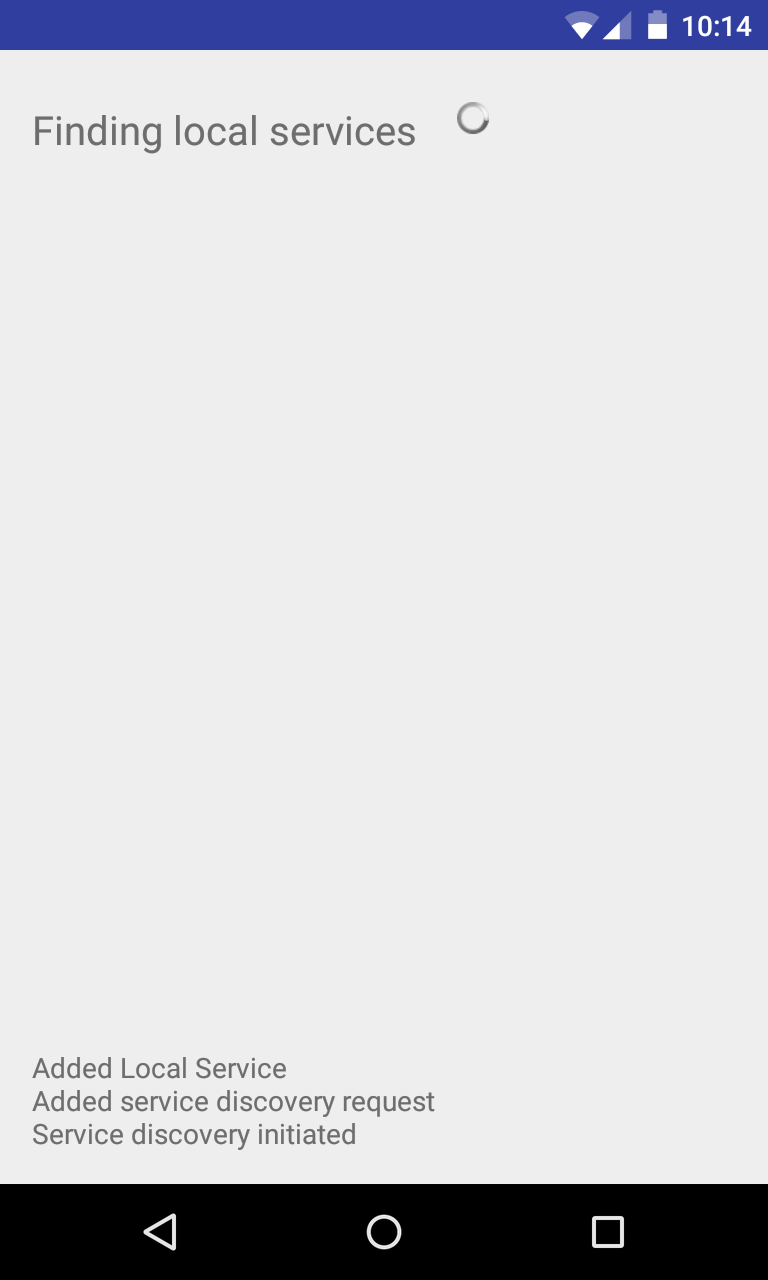
\includegraphics[width=0.5\textwidth]{img}
	\captionof{figure}{Iskanje naprav}
	\label{fig:iskanje_naprav}
\end{minipage}

\section{Zaključek}
%Ali ste izpolnili cilje in možne nadaljne nadgradnje. Pri samem opisu rešitve se običajno sklicujemo na reference, npr. \cite{cisco}. 
Prostora za nadaljne nadgradnje je seveda še ogromno. Lahko bi npr. prenovili uporabniški vmesnik; dodali zvočne signale, ki so nam bolj domači pri uporabi dejanskih walkie-talkiejev; omogočili blokiranje naprav, kar bi pripomoglo tudi k večji varnostni higieni same aplikacije.

Kljub temu so osnovni in glavni cilji aplikacije so izpolnjeni: omogočeno je iskanje naprav, njihovo povezovanje, in prenos zvoka. Obstaja torej nek konkreten temelj, na katerem lahko gradimo naprej.
\pagebreak


\end{document}











